\begin{pa} \label{PA:5.1}
Suppose that the following information is known about a function $f$:  the graph of its derivative, $y = f'(x)$, is given in Figure~\ref{F:5.1.PA1}.  Further, assume that $f'$ is piecewise linear (as pictured) and that for $x \le 0$ and $x \ge 6$, $f'(x) = 0$.  Finally, it is given that $f(0) = 1$.
\begin{figure}[h]
\begin{center}
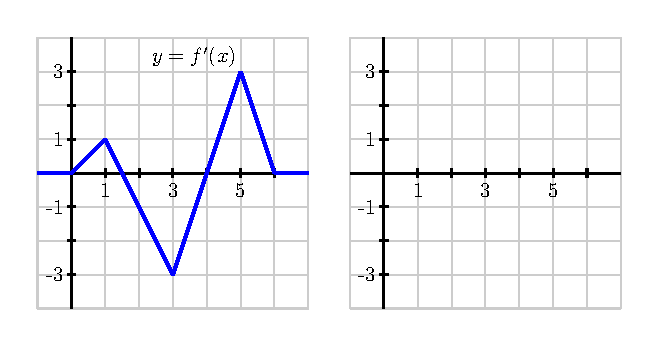
\includegraphics{figures/5_1_PA1.eps}
\caption{At left, the graph of $y = f'(x)$; at right, axes for plotting $y = f(x)$.} \label{F:5.1.PA1}
\end{center}
\end{figure}
\ba
	\item On what interval(s) is $f$ an increasing function?  On what intervals is $f$ decreasing?
	\item On what interval(s) is $f$ concave up?  concave down?
	\item At what point(s) does $f$ have a relative minimum?  a relative maximum?
	\item Recall that the Total Change Theorem tells us that 
$$f(1) - f(0) = \int_0^1 f'(x) \, dx.$$
What is the exact value of $f(1)$?
	\item Use the given information and similar reasoning to that in (d) to determine the exact value of $f(2)$, $f(3)$, $f(4)$, $f(5)$, and $f(6)$.
	\item Based on your responses to all of the preceding questions, sketch a complete and accurate graph of $y = f(x)$ on the axes provided, being sure to indicate the behavior of $f$ for $x < 0$ and $x > 6$.
\ea
\end{pa} 
\afterpa